\documentclass[tikz,border=4pt]{standalone}
\usepackage[utf8]{inputenc}
\usepackage[T1]{fontenc}
\usepackage{lmodern}
\usepackage{amsmath,amssymb}
\usepackage{siunitx}
\sisetup{locale = US, group-separator = {,}}
\usetikzlibrary{calc,positioning}

% Color palette matching thesis standards
\definecolor{colorAixColl}{HTML}{1F77B4}
\definecolor{colorAixP2P}{HTML}{FF7F0E}
\definecolor{colorAixP2PFC}{HTML}{2CA02C}
\definecolor{colorSSZero}{HTML}{D62728}
\definecolor{colorSSThree}{HTML}{9467BD}
\definecolor{colorSSPgdb}{HTML}{8C564B}
\definecolor{colorPhydllDef}{HTML}{008080}
\definecolor{colorPhydllReady}{HTML}{17BECF}

\begin{document}
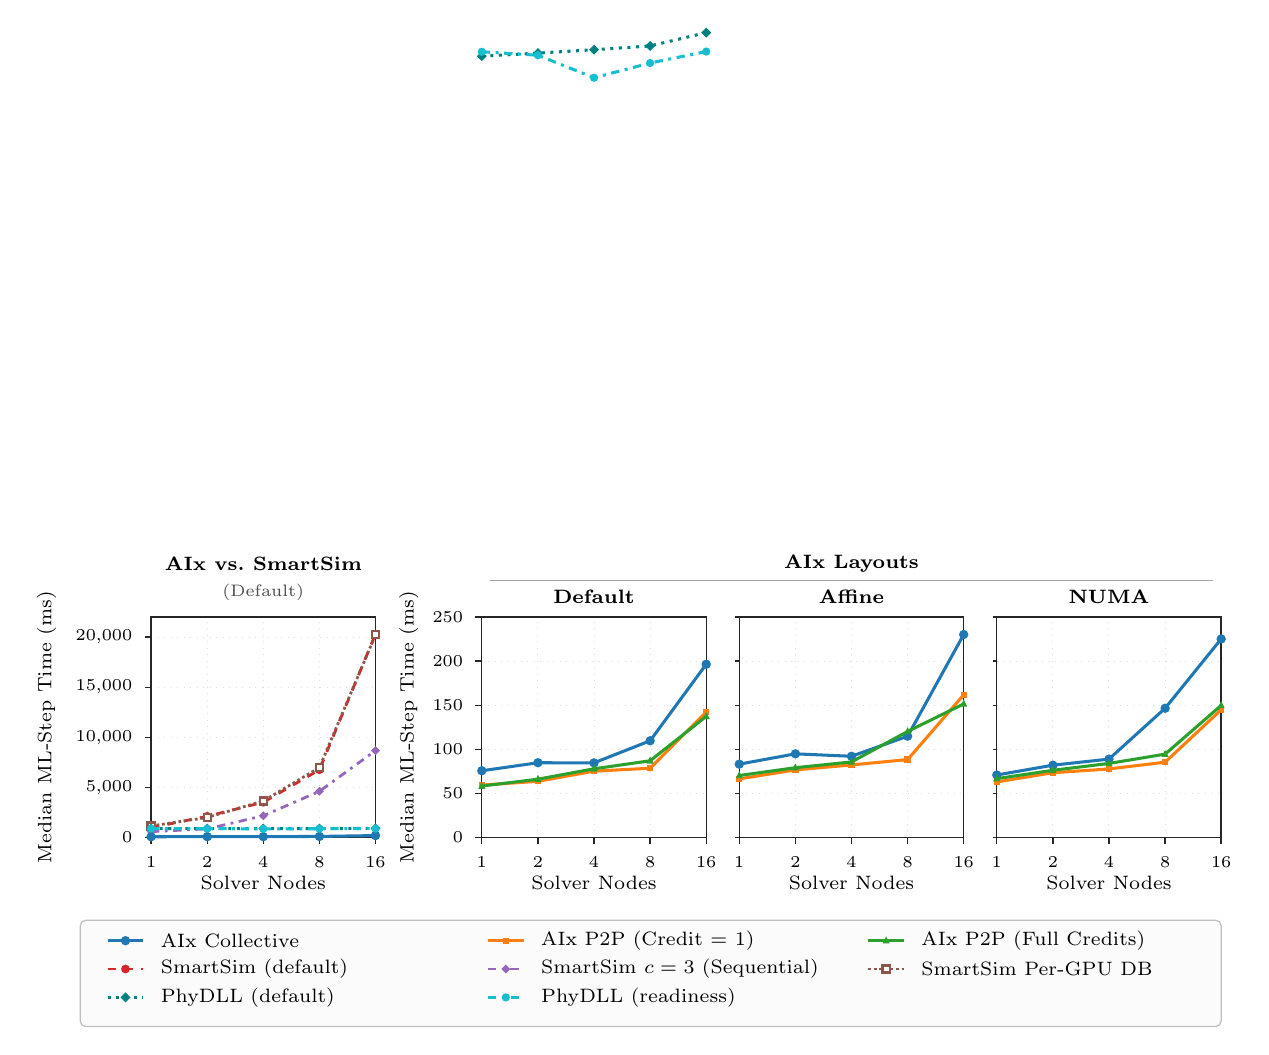
\begin{tikzpicture}[
  font=\fontsize{8}{10}\selectfont,
  axis line/.style={draw=black!85, line width=0.5pt},
  grid line/.style={draw=black!14, line width=0.35pt, dotted},
  tick text/.style={font=\fontsize{6.5}{8}\selectfont},
  main title/.style={font=\fontsize{7.5}{9}\selectfont\bfseries, align=center},
  sub title/.style={font=\fontsize{7.5}{9}\selectfont\bfseries, align=center},
  axis label/.style={font=\fontsize{7}{8.5}\selectfont},
  legend label/.style={font=\fontsize{7}{8.5}\selectfont},
]

% --- Common headline over the 3 AIx subgraphs ---
\node[main title] at (8.895, 3.480) {AIx Layouts};
\draw[draw=black!35, line width=0.4pt] (4.300, 3.260) -- (13.490, 3.260);

% ==================== SUBGRAPH 1 ====================
\begin{scope}[shift={(0.000,0)}]
  \node[main title] at (1.425, 3.480) {AIx vs.\ SmartSim};
  \node[tick text, text=black!70] at (1.425, 3.120) {(Default)};
  \draw[grid line] (0,0.000) -- (2.850,0.000);
  \draw[grid line] (0,0.636) -- (2.850,0.636);
  \draw[grid line] (0,1.273) -- (2.850,1.273);
  \draw[grid line] (0,1.909) -- (2.850,1.909);
  \draw[grid line] (0,2.545) -- (2.850,2.545);
  \draw[grid line] (0.000,0) -- (0.000,2.800);
  \draw[grid line] (0.713,0) -- (0.713,2.800);
  \draw[grid line] (1.425,0) -- (1.425,2.800);
  \draw[grid line] (2.138,0) -- (2.138,2.800);
  \draw[grid line] (2.850,0) -- (2.850,2.800);
  \draw[axis line] (0,0) rectangle (2.850,2.800);
  \draw[axis line] (0.000,0) -- (0.000,-0.08);
  \node[tick text, below=1pt] at (0.000,-0.08) {1};
  \draw[axis line] (0.713,0) -- (0.713,-0.08);
  \node[tick text, below=1pt] at (0.713,-0.08) {2};
  \draw[axis line] (1.425,0) -- (1.425,-0.08);
  \node[tick text, below=1pt] at (1.425,-0.08) {4};
  \draw[axis line] (2.138,0) -- (2.138,-0.08);
  \node[tick text, below=1pt] at (2.138,-0.08) {8};
  \draw[axis line] (2.850,0) -- (2.850,-0.08);
  \node[tick text, below=1pt] at (2.850,-0.08) {16};
  \node[axis label, below=10.5pt] at (1.425,0) {Solver Nodes};
  \draw[axis line] (0,0.000) -- (-0.08,0.000);
  \node[tick text, left=1pt] at (-0.08,0.000) {0};
  \draw[axis line] (0,0.636) -- (-0.08,0.636);
  \node[tick text, left=1pt] at (-0.08,0.636) {5,000};
  \draw[axis line] (0,1.273) -- (-0.08,1.273);
  \node[tick text, left=1pt] at (-0.08,1.273) {10,000};
  \draw[axis line] (0,1.909) -- (-0.08,1.909);
  \node[tick text, left=1pt] at (-0.08,1.909) {15,000};
  \draw[axis line] (0,2.545) -- (-0.08,2.545);
  \node[tick text, left=1pt] at (-0.08,2.545) {20,000};
  \node[axis label, rotate=90, anchor=south] at (-1.08, 1.400) {Median ML-Step Time (ms)};
  \draw[colorSSZero, line width=1.0pt, dashed] (0.000,0.125) -- (0.713,0.270) -- (1.425,0.448) -- (2.138,0.861) -- (2.850,2.584);
  \fill[colorSSZero] (0.000,0.125) circle (1.6pt);
  \fill[colorSSZero] (0.713,0.270) circle (1.6pt);
  \fill[colorSSZero] (1.425,0.448) circle (1.6pt);
  \fill[colorSSZero] (2.138,0.861) circle (1.6pt);
  \fill[colorSSZero] (2.850,2.584) circle (1.6pt);
  \draw[colorSSPgdb, line width=1.0pt, densely dotted] (0.000,0.147) -- (0.713,0.255) -- (1.425,0.464) -- (2.138,0.889) -- (2.850,2.575);
  \draw[colorSSPgdb, line width=0.8pt, fill=white] (-0.045,0.102) rectangle (0.045,0.192);
  \draw[colorSSPgdb, line width=0.8pt, fill=white] (0.667,0.210) rectangle (0.758,0.300);
  \draw[colorSSPgdb, line width=0.8pt, fill=white] (1.380,0.419) rectangle (1.470,0.509);
  \draw[colorSSPgdb, line width=0.8pt, fill=white] (2.093,0.844) rectangle (2.183,0.934);
  \draw[colorSSPgdb, line width=0.8pt, fill=white] (2.805,2.530) rectangle (2.895,2.620);
  \draw[colorSSThree, line width=1.0pt, dashdotted] (0.000,0.075) -- (0.713,0.110) -- (1.425,0.276) -- (2.138,0.587) -- (2.850,1.104);
  \fill[colorSSThree] (0.000,0.075) +(-1.6pt,0) -- +(0,1.6pt) -- +(1.6pt,0) -- +(0,-1.6pt) -- cycle;
  \fill[colorSSThree] (0.713,0.110) +(-1.6pt,0) -- +(0,1.6pt) -- +(1.6pt,0) -- +(0,-1.6pt) -- cycle;
  \fill[colorSSThree] (1.425,0.276) +(-1.6pt,0) -- +(0,1.6pt) -- +(1.6pt,0) -- +(0,-1.6pt) -- cycle;
  \fill[colorSSThree] (2.138,0.587) +(-1.6pt,0) -- +(0,1.6pt) -- +(1.6pt,0) -- +(0,-1.6pt) -- cycle;
  \fill[colorSSThree] (2.850,1.104) +(-1.6pt,0) -- +(0,1.6pt) -- +(1.6pt,0) -- +(0,-1.6pt) -- cycle;
  \draw[colorAixColl, line width=1.1pt] (0.000,0.010) -- (0.713,0.011) -- (1.425,0.011) -- (2.138,0.014) -- (2.850,0.025);
  \fill[colorAixColl] (0.000,0.010) circle (1.7pt);
  \fill[colorAixColl] (0.713,0.011) circle (1.7pt);
  \fill[colorAixColl] (1.425,0.011) circle (1.7pt);
  \fill[colorAixColl] (2.138,0.014) circle (1.7pt);
  \fill[colorAixColl] (2.850,0.025) circle (1.7pt);
  \draw[colorPhydllDef, line width=1.1pt, dotted] (0.000,0.113) -- (0.713,0.113) -- (1.425,0.114) -- (2.138,0.114) -- (2.850,0.116);
  \fill[colorPhydllDef] (0.000,0.113) +(-1.8pt,0) -- +(0,1.8pt) -- +(1.8pt,0) -- +(0,-1.8pt) -- cycle;
  \fill[colorPhydllDef] (0.713,0.113) +(-1.8pt,0) -- +(0,1.8pt) -- +(1.8pt,0) -- +(0,-1.8pt) -- cycle;
  \fill[colorPhydllDef] (1.425,0.114) +(-1.8pt,0) -- +(0,1.8pt) -- +(1.8pt,0) -- +(0,-1.8pt) -- cycle;
  \fill[colorPhydllDef] (2.138,0.114) +(-1.8pt,0) -- +(0,1.8pt) -- +(1.8pt,0) -- +(0,-1.8pt) -- cycle;
  \fill[colorPhydllDef] (2.850,0.116) +(-1.8pt,0) -- +(0,1.8pt) -- +(1.8pt,0) -- +(0,-1.8pt) -- cycle;
  \draw[colorPhydllReady, line width=1.1pt, dashdotted] (0.000,0.113) -- (0.713,0.113) -- (1.425,0.110) -- (2.138,0.112) -- (2.850,0.113);
  \fill[colorPhydllReady] (0.000,0.113) circle (1.5pt);
  \fill[colorPhydllReady] (0.713,0.113) circle (1.5pt);
  \fill[colorPhydllReady] (1.425,0.110) circle (1.5pt);
  \fill[colorPhydllReady] (2.138,0.112) circle (1.5pt);
  \fill[colorPhydllReady] (2.850,0.113) circle (1.5pt);
\end{scope}

% ==================== SUBGRAPH 2 ====================
\begin{scope}[shift={(4.200,0)}]
  \node[sub title] at (1.425, 3.060) {Default};
  \draw[grid line] (0,0.000) -- (2.850,0.000);
  \draw[grid line] (0,0.560) -- (2.850,0.560);
  \draw[grid line] (0,1.120) -- (2.850,1.120);
  \draw[grid line] (0,1.680) -- (2.850,1.680);
  \draw[grid line] (0,2.240) -- (2.850,2.240);
  \draw[grid line] (0,2.800) -- (2.850,2.800);
  \draw[grid line] (0.000,0) -- (0.000,2.800);
  \draw[grid line] (0.713,0) -- (0.713,2.800);
  \draw[grid line] (1.425,0) -- (1.425,2.800);
  \draw[grid line] (2.138,0) -- (2.138,2.800);
  \draw[grid line] (2.850,0) -- (2.850,2.800);
  \draw[axis line] (0,0) rectangle (2.850,2.800);
  \draw[axis line] (0.000,0) -- (0.000,-0.08);
  \node[tick text, below=1pt] at (0.000,-0.08) {1};
  \draw[axis line] (0.713,0) -- (0.713,-0.08);
  \node[tick text, below=1pt] at (0.713,-0.08) {2};
  \draw[axis line] (1.425,0) -- (1.425,-0.08);
  \node[tick text, below=1pt] at (1.425,-0.08) {4};
  \draw[axis line] (2.138,0) -- (2.138,-0.08);
  \node[tick text, below=1pt] at (2.138,-0.08) {8};
  \draw[axis line] (2.850,0) -- (2.850,-0.08);
  \node[tick text, below=1pt] at (2.850,-0.08) {16};
  \node[axis label, below=10.5pt] at (1.425,0) {Solver Nodes};
  \draw[axis line] (0,0.000) -- (-0.08,0.000);
  \node[tick text, left=1pt] at (-0.08,0.000) {0};
  \draw[axis line] (0,0.560) -- (-0.08,0.560);
  \node[tick text, left=1pt] at (-0.08,0.560) {50};
  \draw[axis line] (0,1.120) -- (-0.08,1.120);
  \node[tick text, left=1pt] at (-0.08,1.120) {100};
  \draw[axis line] (0,1.680) -- (-0.08,1.680);
  \node[tick text, left=1pt] at (-0.08,1.680) {150};
  \draw[axis line] (0,2.240) -- (-0.08,2.240);
  \node[tick text, left=1pt] at (-0.08,2.240) {200};
  \draw[axis line] (0,2.800) -- (-0.08,2.800);
  \node[tick text, left=1pt] at (-0.08,2.800) {250};
  \node[axis label, rotate=90, anchor=south] at (-0.68, 1.400) {Median ML-Step Time (ms)};
  \draw[colorAixColl, line width=1.1pt] (0.000,0.848) -- (0.713,0.950) -- (1.425,0.948) -- (2.138,1.229) -- (2.850,2.201);
  \fill[colorAixColl] (0.000,0.848) circle (1.7pt);
  \fill[colorAixColl] (0.713,0.950) circle (1.7pt);
  \fill[colorAixColl] (1.425,0.948) circle (1.7pt);
  \fill[colorAixColl] (2.138,1.229) circle (1.7pt);
  \fill[colorAixColl] (2.850,2.201) circle (1.7pt);
  \draw[colorAixP2P, line width=1.1pt] (0.000,0.666) -- (0.713,0.714) -- (1.425,0.843) -- (2.138,0.880) -- (2.850,1.595);
  \fill[colorAixP2P] (-0.040,0.626) rectangle (0.040,0.706);
  \fill[colorAixP2P] (0.672,0.674) rectangle (0.753,0.754);
  \fill[colorAixP2P] (1.385,0.803) rectangle (1.465,0.883);
  \fill[colorAixP2P] (2.098,0.840) rectangle (2.178,0.920);
  \fill[colorAixP2P] (2.810,1.555) rectangle (2.890,1.635);
  \draw[colorAixP2PFC, line width=1.1pt] (0.000,0.654) -- (0.713,0.741) -- (1.425,0.873) -- (2.138,0.975) -- (2.850,1.539);
  \fill[colorAixP2PFC] (0.000,0.709) -- (-0.045,0.619) -- (0.045,0.619) -- cycle;
  \fill[colorAixP2PFC] (0.713,0.796) -- (0.667,0.706) -- (0.758,0.706) -- cycle;
  \fill[colorAixP2PFC] (1.425,0.928) -- (1.380,0.838) -- (1.470,0.838) -- cycle;
  \fill[colorAixP2PFC] (2.138,1.030) -- (2.093,0.940) -- (2.183,0.940) -- cycle;
  \fill[colorAixP2PFC] (2.850,1.594) -- (2.805,1.504) -- (2.895,1.504) -- cycle;
  \draw[colorPhydllDef, line width=1.1pt, dotted] (0.000,9.923) -- (0.713,9.962) -- (1.425,10.005) -- (2.138,10.053) -- (2.850,10.222);
  \fill[colorPhydllDef] (0.000,9.923) +(-1.8pt,0) -- +(0,1.8pt) -- +(1.8pt,0) -- +(0,-1.8pt) -- cycle;
  \fill[colorPhydllDef] (0.713,9.962) +(-1.8pt,0) -- +(0,1.8pt) -- +(1.8pt,0) -- +(0,-1.8pt) -- cycle;
  \fill[colorPhydllDef] (1.425,10.005) +(-1.8pt,0) -- +(0,1.8pt) -- +(1.8pt,0) -- +(0,-1.8pt) -- cycle;
  \fill[colorPhydllDef] (2.138,10.053) +(-1.8pt,0) -- +(0,1.8pt) -- +(1.8pt,0) -- +(0,-1.8pt) -- cycle;
  \fill[colorPhydllDef] (2.850,10.222) +(-1.8pt,0) -- +(0,1.8pt) -- +(1.8pt,0) -- +(0,-1.8pt) -- cycle;
  \draw[colorPhydllReady, line width=1.1pt, dashdotted] (0.000,9.979) -- (0.713,9.935) -- (1.425,9.649) -- (2.138,9.836) -- (2.850,9.982);
  \fill[colorPhydllReady] (0.000,9.979) circle (1.5pt);
  \fill[colorPhydllReady] (0.713,9.935) circle (1.5pt);
  \fill[colorPhydllReady] (1.425,9.649) circle (1.5pt);
  \fill[colorPhydllReady] (2.138,9.836) circle (1.5pt);
  \fill[colorPhydllReady] (2.850,9.982) circle (1.5pt);
\end{scope}

% ==================== SUBGRAPH 3 ====================
\begin{scope}[shift={(7.470,0)}]
  \node[sub title] at (1.425, 3.060) {Affine};
  \draw[grid line] (0,0.000) -- (2.850,0.000);
  \draw[grid line] (0,0.560) -- (2.850,0.560);
  \draw[grid line] (0,1.120) -- (2.850,1.120);
  \draw[grid line] (0,1.680) -- (2.850,1.680);
  \draw[grid line] (0,2.240) -- (2.850,2.240);
  \draw[grid line] (0,2.800) -- (2.850,2.800);
  \draw[grid line] (0.000,0) -- (0.000,2.800);
  \draw[grid line] (0.713,0) -- (0.713,2.800);
  \draw[grid line] (1.425,0) -- (1.425,2.800);
  \draw[grid line] (2.138,0) -- (2.138,2.800);
  \draw[grid line] (2.850,0) -- (2.850,2.800);
  \draw[axis line] (0,0) rectangle (2.850,2.800);
  \draw[axis line] (0.000,0) -- (0.000,-0.08);
  \node[tick text, below=1pt] at (0.000,-0.08) {1};
  \draw[axis line] (0.713,0) -- (0.713,-0.08);
  \node[tick text, below=1pt] at (0.713,-0.08) {2};
  \draw[axis line] (1.425,0) -- (1.425,-0.08);
  \node[tick text, below=1pt] at (1.425,-0.08) {4};
  \draw[axis line] (2.138,0) -- (2.138,-0.08);
  \node[tick text, below=1pt] at (2.138,-0.08) {8};
  \draw[axis line] (2.850,0) -- (2.850,-0.08);
  \node[tick text, below=1pt] at (2.850,-0.08) {16};
  \node[axis label, below=10.5pt] at (1.425,0) {Solver Nodes};
  \draw[axis line] (0,0.000) -- (-0.05,0.000);
  \draw[axis line] (0,0.560) -- (-0.05,0.560);
  \draw[axis line] (0,1.120) -- (-0.05,1.120);
  \draw[axis line] (0,1.680) -- (-0.05,1.680);
  \draw[axis line] (0,2.240) -- (-0.05,2.240);
  \draw[axis line] (0,2.800) -- (-0.05,2.800);
  \draw[colorAixColl, line width=1.1pt] (0.000,0.932) -- (0.713,1.063) -- (1.425,1.032) -- (2.138,1.287) -- (2.850,2.578);
  \fill[colorAixColl] (0.000,0.932) circle (1.7pt);
  \fill[colorAixColl] (0.713,1.063) circle (1.7pt);
  \fill[colorAixColl] (1.425,1.032) circle (1.7pt);
  \fill[colorAixColl] (2.138,1.287) circle (1.7pt);
  \fill[colorAixColl] (2.850,2.578) circle (1.7pt);
  \draw[colorAixP2P, line width=1.1pt] (0.000,0.745) -- (0.713,0.859) -- (1.425,0.922) -- (2.138,0.990) -- (2.850,1.812);
  \fill[colorAixP2P] (-0.040,0.705) rectangle (0.040,0.785);
  \fill[colorAixP2P] (0.672,0.819) rectangle (0.753,0.899);
  \fill[colorAixP2P] (1.385,0.882) rectangle (1.465,0.962);
  \fill[colorAixP2P] (2.098,0.950) rectangle (2.178,1.030);
  \fill[colorAixP2P] (2.810,1.772) rectangle (2.890,1.852);
  \draw[colorAixP2PFC, line width=1.1pt] (0.000,0.788) -- (0.713,0.887) -- (1.425,0.960) -- (2.138,1.347) -- (2.850,1.697);
  \fill[colorAixP2PFC] (0.000,0.843) -- (-0.045,0.753) -- (0.045,0.753) -- cycle;
  \fill[colorAixP2PFC] (0.713,0.942) -- (0.667,0.852) -- (0.758,0.852) -- cycle;
  \fill[colorAixP2PFC] (1.425,1.015) -- (1.380,0.925) -- (1.470,0.925) -- cycle;
  \fill[colorAixP2PFC] (2.138,1.402) -- (2.093,1.312) -- (2.183,1.312) -- cycle;
  \fill[colorAixP2PFC] (2.850,1.752) -- (2.805,1.662) -- (2.895,1.662) -- cycle;
\end{scope}

% ==================== SUBGRAPH 4 ====================
\begin{scope}[shift={(10.740,0)}]
  \node[sub title] at (1.425, 3.060) {NUMA};
  \draw[grid line] (0,0.000) -- (2.850,0.000);
  \draw[grid line] (0,0.560) -- (2.850,0.560);
  \draw[grid line] (0,1.120) -- (2.850,1.120);
  \draw[grid line] (0,1.680) -- (2.850,1.680);
  \draw[grid line] (0,2.240) -- (2.850,2.240);
  \draw[grid line] (0,2.800) -- (2.850,2.800);
  \draw[grid line] (0.000,0) -- (0.000,2.800);
  \draw[grid line] (0.713,0) -- (0.713,2.800);
  \draw[grid line] (1.425,0) -- (1.425,2.800);
  \draw[grid line] (2.138,0) -- (2.138,2.800);
  \draw[grid line] (2.850,0) -- (2.850,2.800);
  \draw[axis line] (0,0) rectangle (2.850,2.800);
  \draw[axis line] (0.000,0) -- (0.000,-0.08);
  \node[tick text, below=1pt] at (0.000,-0.08) {1};
  \draw[axis line] (0.713,0) -- (0.713,-0.08);
  \node[tick text, below=1pt] at (0.713,-0.08) {2};
  \draw[axis line] (1.425,0) -- (1.425,-0.08);
  \node[tick text, below=1pt] at (1.425,-0.08) {4};
  \draw[axis line] (2.138,0) -- (2.138,-0.08);
  \node[tick text, below=1pt] at (2.138,-0.08) {8};
  \draw[axis line] (2.850,0) -- (2.850,-0.08);
  \node[tick text, below=1pt] at (2.850,-0.08) {16};
  \node[axis label, below=10.5pt] at (1.425,0) {Solver Nodes};
  \draw[axis line] (0,0.000) -- (-0.05,0.000);
  \draw[axis line] (0,0.560) -- (-0.05,0.560);
  \draw[axis line] (0,1.120) -- (-0.05,1.120);
  \draw[axis line] (0,1.680) -- (-0.05,1.680);
  \draw[axis line] (0,2.240) -- (-0.05,2.240);
  \draw[axis line] (0,2.800) -- (-0.05,2.800);
  \draw[colorAixColl, line width=1.1pt] (0.000,0.794) -- (0.713,0.919) -- (1.425,0.996) -- (2.138,1.642) -- (2.850,2.522);
  \fill[colorAixColl] (0.000,0.794) circle (1.7pt);
  \fill[colorAixColl] (0.713,0.919) circle (1.7pt);
  \fill[colorAixColl] (1.425,0.996) circle (1.7pt);
  \fill[colorAixColl] (2.138,1.642) circle (1.7pt);
  \fill[colorAixColl] (2.850,2.522) circle (1.7pt);
  \draw[colorAixP2P, line width=1.1pt] (0.000,0.706) -- (0.713,0.823) -- (1.425,0.871) -- (2.138,0.957) -- (2.850,1.623);
  \fill[colorAixP2P] (-0.040,0.666) rectangle (0.040,0.746);
  \fill[colorAixP2P] (0.672,0.783) rectangle (0.753,0.863);
  \fill[colorAixP2P] (1.385,0.831) rectangle (1.465,0.911);
  \fill[colorAixP2P] (2.098,0.917) rectangle (2.178,0.997);
  \fill[colorAixP2P] (2.810,1.583) rectangle (2.890,1.663);
  \draw[colorAixP2PFC, line width=1.1pt] (0.000,0.748) -- (0.713,0.854) -- (1.425,0.941) -- (2.138,1.059) -- (2.850,1.678);
  \fill[colorAixP2PFC] (0.000,0.803) -- (-0.045,0.713) -- (0.045,0.713) -- cycle;
  \fill[colorAixP2PFC] (0.713,0.909) -- (0.667,0.819) -- (0.758,0.819) -- cycle;
  \fill[colorAixP2PFC] (1.425,0.996) -- (1.380,0.906) -- (1.470,0.906) -- cycle;
  \fill[colorAixP2PFC] (2.138,1.114) -- (2.093,1.024) -- (2.183,1.024) -- cycle;
  \fill[colorAixP2PFC] (2.850,1.733) -- (2.805,1.643) -- (2.895,1.643) -- cycle;
\end{scope}

% ==================== SHARED LEGEND ====================
\begin{scope}[shift={(0,-1.050)}]
  \draw[draw=black!25, fill=gray!3, rounded corners=2pt, line width=0.45pt]
    (-0.900, -1.350) rectangle (13.590, 0);
  \draw[colorAixColl, line width=1.1pt] (-0.550,-0.26) -- (-0.100,-0.26);
  \fill[colorAixColl] (-0.325,-0.26) circle (1.7pt);
  \node[legend label, anchor=west] at (0.000,-0.26) {AIx Collective};
  \draw[colorAixP2P, line width=1.1pt] (4.280,-0.26) -- (4.730,-0.26);
  \fill[colorAixP2P] (4.465,-0.300) rectangle (4.545,-0.220);
  \node[legend label, anchor=west] at (4.830,-0.26) {AIx P2P (Credit = 1)};
  \draw[colorAixP2PFC, line width=1.1pt] (9.110,-0.26) -- (9.560,-0.26);
  \fill[colorAixP2PFC] (9.335,-0.205) -- (9.290,-0.295) -- (9.380,-0.295) -- cycle;
  \node[legend label, anchor=west] at (9.660,-0.26) {AIx P2P (Full Credits)};
  \draw[colorSSZero, line width=1.0pt, dashed] (-0.550,-0.62) -- (-0.100,-0.62);
  \fill[colorSSZero] (-0.325,-0.62) circle (1.6pt);
  \node[legend label, anchor=west] at (0.000,-0.62) {SmartSim (default)};
  \draw[colorSSThree, line width=1.0pt, dashdotted] (4.280,-0.62) -- (4.730,-0.62);
  \fill[colorSSThree] (4.505,-0.62) +(-1.6pt,0) -- +(0,1.6pt) -- +(1.6pt,0) -- +(0,-1.6pt) -- cycle;
  \node[legend label, anchor=west] at (4.830,-0.62) {SmartSim $c=3$ (Sequential)};
  \draw[colorSSPgdb, line width=1.0pt, densely dotted] (9.110,-0.62) -- (9.560,-0.62);
  \draw[colorSSPgdb, line width=0.8pt, fill=white] (9.290,-0.665) rectangle (9.380,-0.575);
  \node[legend label, anchor=west] at (9.660,-0.62) {SmartSim Per-GPU DB};
  \draw[colorPhydllDef, line width=1.1pt, dotted] (-0.550,-0.98) -- (-0.100,-0.98);
  \fill[colorPhydllDef] (-0.325,-0.98) +(-1.8pt,0) -- +(0,1.8pt) -- +(1.8pt,0) -- +(0,-1.8pt) -- cycle;
  \node[legend label, anchor=west] at (0.000,-0.98) {PhyDLL (default)};
  \draw[colorPhydllReady, line width=1.1pt, dashdotted] (4.280,-0.98) -- (4.730,-0.98);
  \fill[colorPhydllReady] (4.505,-0.98) circle (1.5pt);
  \node[legend label, anchor=west] at (4.830,-0.98) {PhyDLL (readiness)};
\end{scope}
\end{tikzpicture}
\end{document}
